\begin{tabular}{p{0.5\textwidth} p{0.5\textwidth}}
  \tablesubsection{Work Done by a Varying Force}
  \label{ssec:varying_force_work}
   & \\%adds spacing stuff
\end{tabular}

\pgfplotsset{%DEFINES INTEGRAL STUFF
  integral segments/.code={\pgfmathsetmacro\integralsegments{#1}},
  integral segments=40,%modify to adjust number of rectangles
  integral/.style args={#1:#2}{
    ybar interval,
    domain=#1+((#2-#1)/\integralsegments)/2:#2+((#2-#1)/\integralsegments)/2,
    samples=\integralsegments+1,
    x filter/.code=\pgfmathparse{\pgfmathresult-((#2-#1)/\integralsegments)/2}
  }
}

\begin{center}
  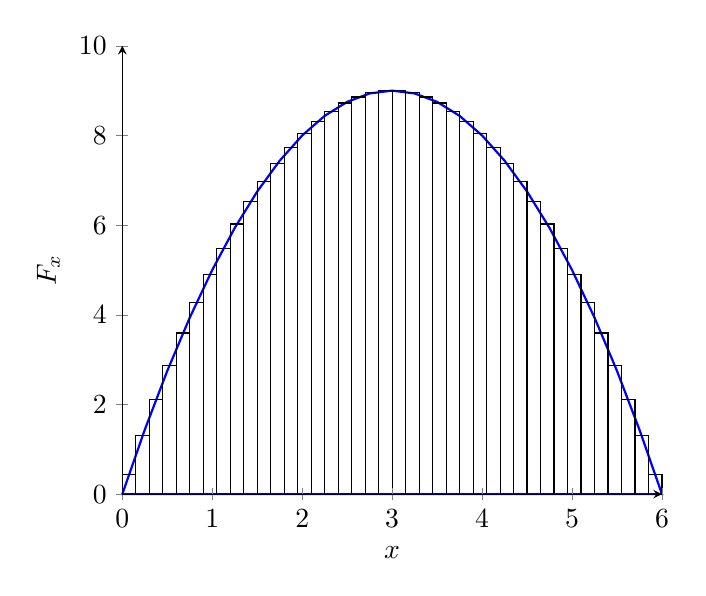
\begin{tikzpicture}
    \begin{axis}[
      xlabel=$x$,
      ylabel=$F_x$,
      xtick={0,1,2,3,4,5,6},
      ytick={0,2,4,6,8,10},
      xmax=6, ymax=10, ymin=0, xmin=0,
      enlargelimits=true,
      axis lines=left,
      clip=false,
      domain=0:6,
      axis on top
      ]

      \addplot[mark=none, color=blue, thick]{-(x-3)^2+9}\closedcycle;%formula to represent integral
      \addplot[integral=0:6]{-(x-3)^2+9};
    \end{axis}
  \end{tikzpicture}
\end{center}  

The above is a graph of the varying force $F_x$ across a distance $x$ with Riemann sums approximating its integral. Each rectangle has a length equal to the magnitude of $F_x$ and a width equal to the small distance $x_i$. \\

%VARYING FORCE MATH

The following formula yields the work done by a varying force $F_x$ described above. In this formula, $F_i$ is the magnitude of the varying force $F_x$ at the midpoint of a small distance $\Delta x_i$, the width of one of a number of infinitely small rectangles whose area may be approximated $A = \ell w = F_i\Delta x_i$.

\[ W \cong \sum_{i=1}^{\infty} F_i \Delta x_i \]

The definite integral found below is an alternate representation of the above Riemann sum, approximating the work performed by a force $F_x$ at each point $x$ across the distance $\Delta x = x_f - x_i$.

\[ \int_{x_i}^{x_f} F_x \]
%%% Local Variables:
%%% mode: latex
%%% TeX-master: "../main"
%%% End: